\documentclass{article}
\usepackage{times}
\usepackage{amsmath,amssymb}
\usepackage{tikz}
\pdfpagewidth=12.7cm
\pdfpageheight=6.8cm
\setlength{\paperwidth}{12.7cm}
\setlength{\paperheight}{6.8cm}
\setlength{\oddsidemargin}{-1in}
\setlength{\evensidemargin}{-1in}
\setlength{\topmargin}{-1in}
\setlength{\headheight}{0pt}
\setlength{\headsep}{0pt}
\setlength{\textwidth}{12.7cm}
\setlength{\textheight}{6.8cm}
\pagestyle{empty}
\tikzset{every picture/.style={line width=0.5pt}}

\begin{document}
\noindent\resizebox{\linewidth}{!}{%
\begin{tikzpicture}[x=1cm,y=1cm,baseline=(current bounding box.north)]
\node at (2.95,4.62) {\small (a) discrete coefficients $(J_2)$};
\node at (2.95,4.22) {\scriptsize any single strut suffices to hold the beam};
\fill[black!12] (0.15,3.30) rectangle (5.75,3.95);
\draw (0.15,3.30) rectangle (5.75,3.95);
\node at (2.95,3.625) {\small $G$ is affine};
\foreach \cx/\lab in {0.62/{continuity}, 1.78/{measurability},
  2.95/{monotonicity}, 4.12/{bdd.\ on $E$, $|E|{>}0$}, 5.28/{bdd.\ on $I$}}{
  \fill[black!6] (\cx-0.23,0.90) rectangle (\cx+0.23,3.30);
  \draw (\cx-0.23,0.90) rectangle (\cx+0.23,3.30);
  \node[rotate=90] at (\cx,2.10) {\scriptsize \lab};
}
\draw[thick] (0,0.90) -- (5.9,0.90);
\foreach \x in {0.15,0.45,...,5.85}{\draw[black!60] (\x,0.90) -- (\x-0.16,0.70);}
\node[align=center] at (2.95,0.30)
  {\scriptsize remove every strut and the beam falls:\\[-1pt]
   \scriptsize Hamel pathology (Proposition 7)};
\draw[black!30] (6.32,0.05) -- (6.32,4.80);
\node at (9.65,4.62) {\small (b) continuous coefficients $(\star)$};
\node at (9.65,4.22) {\scriptsize no strut needed; each becomes a conclusion (Corollary 2)};
\fill[black!12] (6.85,3.30) rectangle (12.45,3.95);
\draw (6.85,3.30) rectangle (12.45,3.95);
\node at (9.65,3.625) {\small $G$ is affine};
\foreach \cx in {7.12, 7.95, 8.78, 10.82, 11.98}{
  \draw[black!45, dash pattern=on 2pt off 2pt] (\cx-0.23,0.90) rectangle (\cx+0.23,3.30);
}
\node[black!55, rotate=90] at (7.12,2.10) {\scriptsize removed};
\node[black!55, rotate=90] at (7.95,2.10) {\scriptsize removed};
\node[black!55, rotate=90] at (8.78,2.10) {\scriptsize removed};
\node[black!55, rotate=90] at (10.82,2.10) {\scriptsize removed};
\node[black!55, rotate=90] at (11.98,2.10) {\scriptsize removed};
\fill[black!25] (9.22,0.90) rectangle (10.08,3.30);
\draw (9.22,0.90) rectangle (10.08,3.30);
\node[rotate=90] at (9.65,2.10) {\scriptsize Theorem 1};
\draw[thick] (6.7,0.90) -- (12.6,0.90);
\foreach \x in {6.85,7.15,...,12.55}{\draw[black!60] (\x,0.90) -- (\x-0.16,0.70);}
\node[align=center] at (9.65,0.30)
  {\scriptsize no pathology survives below ground:\\[-1pt]
   \scriptsize $(\star)$ tests every irrational weight};
\end{tikzpicture}%
}%
\end{document}